\documentclass[14pt]{extbook}
\usepackage{multicol, enumerate, enumitem, hyperref, color, soul, setspace, parskip, fancyhdr} %General Packages
\usepackage{amssymb, amsthm, amsmath, bbm, latexsym, units, mathtools} %Math Packages
\everymath{\displaystyle} %All math in Display Style
% Packages with additional options
\usepackage[headsep=0.5cm,headheight=12pt, left=1 in,right= 1 in,top= 1 in,bottom= 1 in]{geometry}
\usepackage[usenames,dvipsnames]{xcolor}
\usepackage{dashrule}  % Package to use the command below to create lines between items
\newcommand{\litem}[1]{\item#1\hspace*{-1cm}\rule{\textwidth}{0.4pt}}
\pagestyle{fancy}
\lhead{Progress Quiz 8}
\chead{}
\rhead{Version B}
\lfoot{4553-3922}
\cfoot{}
\rfoot{Fall 2020}
\begin{document}

\begin{enumerate}
\litem{
Describe the end behavior of the polynomial below.\[ f(x) = 7(x + 2)^{2}(x - 2)^{3}(x + 8)^{2}(x - 8)^{4} \]\begin{enumerate}[label=\Alph*.]
\begin{multicols}{2}\item 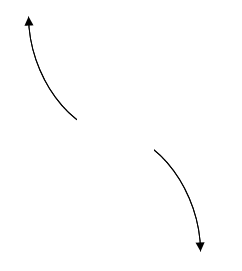
\includegraphics[width = 0.3\textwidth]{../Figures/polyEndBehaviorAB.png}\item 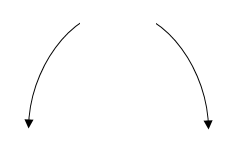
\includegraphics[width = 0.3\textwidth]{../Figures/polyEndBehaviorBB.png}\item 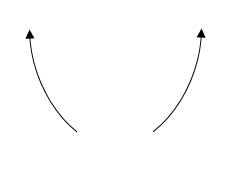
\includegraphics[width = 0.3\textwidth]{../Figures/polyEndBehaviorCB.png}\item 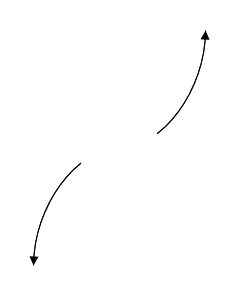
\includegraphics[width = 0.3\textwidth]{../Figures/polyEndBehaviorDB.png}\end{multicols}\item None of the above.
\end{enumerate} }
\litem{
Construct the lowest-degree polynomial given the zeros below. Then, choose the intervals that contain the coefficients of the polynomial in the form $ax^3+bx^2+cx+d$.\[ \frac{-7}{5}, \frac{-4}{5}, \text{ and } 5 \]\begin{enumerate}[label=\Alph*.]
\item \( a \in [19, 30], b \in [-70, -63], c \in [-249, -243], \text{ and } d \in [-143, -137] \)
\item \( a \in [19, 30], b \in [-187, -178], c \in [302, 305], \text{ and } d \in [-143, -137] \)
\item \( a \in [19, 30], b \in [62, 76], c \in [-249, -243], \text{ and } d \in [140, 144] \)
\item \( a \in [19, 30], b \in [-143, -137], c \in [45, 48], \text{ and } d \in [140, 144] \)
\item \( a \in [19, 30], b \in [-70, -63], c \in [-249, -243], \text{ and } d \in [140, 144] \)

\end{enumerate} }
\litem{
Describe the zero behavior of the zero $x = -6$ of the polynomial below.\[ f(x) = 4(x - 6)^{5}(x + 6)^{10}(x + 3)^{7}(x - 3)^{9} \]\begin{enumerate}[label=\Alph*.]
\begin{multicols}{2}\item 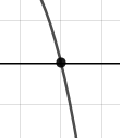
\includegraphics[width = 0.3\textwidth]{../Figures/polyZeroBehaviorCopyAB.png}\item 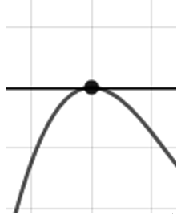
\includegraphics[width = 0.3\textwidth]{../Figures/polyZeroBehaviorCopyBB.png}\item 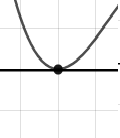
\includegraphics[width = 0.3\textwidth]{../Figures/polyZeroBehaviorCopyCB.png}\item 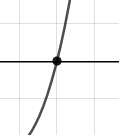
\includegraphics[width = 0.3\textwidth]{../Figures/polyZeroBehaviorCopyDB.png}\end{multicols}\item None of the above.
\end{enumerate} }
\litem{
Construct the lowest-degree polynomial given the zeros below. Then, choose the intervals that contain the coefficients of the polynomial in the form $x^3+bx^2+cx+d$.\[ 5 - 5 i \text{ and } 2 \]\begin{enumerate}[label=\Alph*.]
\item \( b \in [1, 7], c \in [0, 9], \text{ and } d \in [-11, -9] \)
\item \( b \in [1, 7], c \in [-14, -5], \text{ and } d \in [8, 12] \)
\item \( b \in [-20, -8], c \in [63, 71], \text{ and } d \in [-104, -92] \)
\item \( b \in [11, 17], c \in [63, 71], \text{ and } d \in [98, 106] \)
\item \( \text{None of the above.} \)

\end{enumerate} }
\litem{
Which of the following equations \textit{could} be of the graph presented below?
\begin{center}
    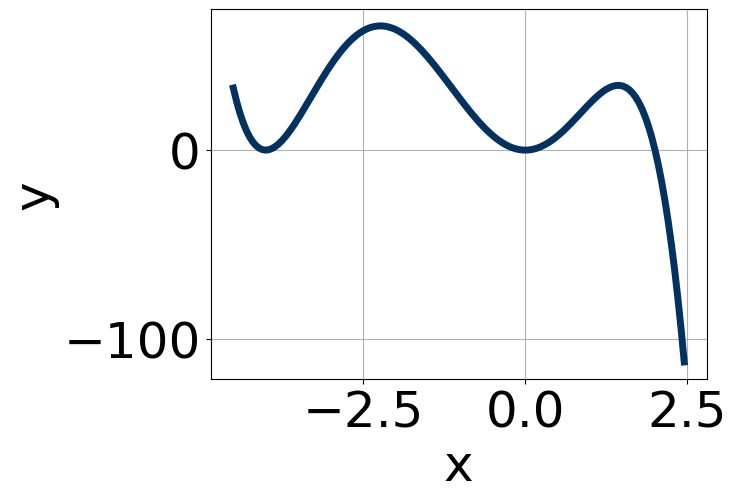
\includegraphics[width=0.5\textwidth]{../Figures/polyGraphToFunctionCopyB.png}
\end{center}
\begin{enumerate}[label=\Alph*.]
\item \( -12x^{4} (x + 4)^{8} (x - 2)^{7} \)
\item \( -11x^{9} (x + 4)^{10} (x - 2)^{9} \)
\item \( 4x^{4} (x + 4)^{8} (x - 2)^{9} \)
\item \( 11x^{8} (x + 4)^{4} (x - 2)^{8} \)
\item \( -12x^{9} (x + 4)^{8} (x - 2)^{4} \)

\end{enumerate} }
\litem{
Describe the zero behavior of the zero $x = 4$ of the polynomial below.\[ f(x) = 3(x - 3)^{8}(x + 3)^{4}(x + 4)^{8}(x - 4)^{5} \]\begin{enumerate}[label=\Alph*.]
\begin{multicols}{2}\item 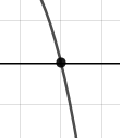
\includegraphics[width = 0.3\textwidth]{../Figures/polyZeroBehaviorAB.png}\item 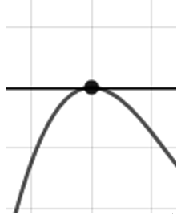
\includegraphics[width = 0.3\textwidth]{../Figures/polyZeroBehaviorBB.png}\item 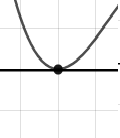
\includegraphics[width = 0.3\textwidth]{../Figures/polyZeroBehaviorCB.png}\item 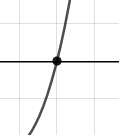
\includegraphics[width = 0.3\textwidth]{../Figures/polyZeroBehaviorDB.png}\end{multicols}\item None of the above.
\end{enumerate} }
\litem{
Describe the end behavior of the polynomial below.\[ f(x) = -8(x + 9)^{2}(x - 9)^{7}(x + 5)^{5}(x - 5)^{6} \]\begin{enumerate}[label=\Alph*.]
\begin{multicols}{2}\item 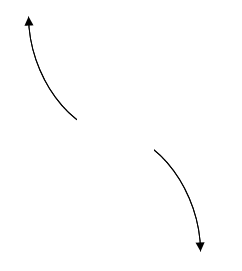
\includegraphics[width = 0.3\textwidth]{../Figures/polyEndBehaviorCopyAB.png}\item 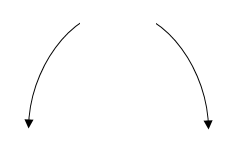
\includegraphics[width = 0.3\textwidth]{../Figures/polyEndBehaviorCopyBB.png}\item 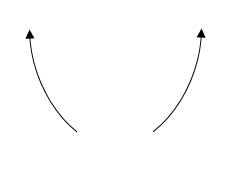
\includegraphics[width = 0.3\textwidth]{../Figures/polyEndBehaviorCopyCB.png}\item 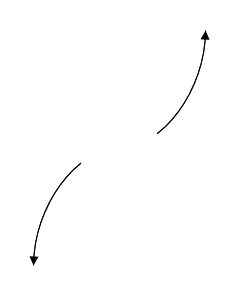
\includegraphics[width = 0.3\textwidth]{../Figures/polyEndBehaviorCopyDB.png}\end{multicols}\item None of the above.
\end{enumerate} }
\litem{
Construct the lowest-degree polynomial given the zeros below. Then, choose the intervals that contain the coefficients of the polynomial in the form $x^3+bx^2+cx+d$.\[ -5 + 3 i \text{ and } 4 \]\begin{enumerate}[label=\Alph*.]
\item \( b \in [0, 4], c \in [-2.1, 2], \text{ and } d \in [-25, -13] \)
\item \( b \in [0, 4], c \in [-7.1, -6.5], \text{ and } d \in [10, 14] \)
\item \( b \in [4, 15], c \in [-6.9, -5.4], \text{ and } d \in [-140, -129] \)
\item \( b \in [-11, -4], c \in [-6.9, -5.4], \text{ and } d \in [136, 144] \)
\item \( \text{None of the above.} \)

\end{enumerate} }
\litem{
Construct the lowest-degree polynomial given the zeros below. Then, choose the intervals that contain the coefficients of the polynomial in the form $ax^3+bx^2+cx+d$.\[ \frac{-1}{3}, \frac{-6}{5}, \text{ and } \frac{4}{3} \]\begin{enumerate}[label=\Alph*.]
\item \( a \in [45, 55], b \in [9, 16], c \in [-77.5, -73.9], \text{ and } d \in [21, 28] \)
\item \( a \in [45, 55], b \in [9, 16], c \in [-77.5, -73.9], \text{ and } d \in [-24, -21] \)
\item \( a \in [45, 55], b \in [-13, -5], c \in [-77.5, -73.9], \text{ and } d \in [21, 28] \)
\item \( a \in [45, 55], b \in [-24, -13], c \in [-73.1, -67.6], \text{ and } d \in [21, 28] \)
\item \( a \in [45, 55], b \in [-130, -126], c \in [109, 113], \text{ and } d \in [-24, -21] \)

\end{enumerate} }
\litem{
Which of the following equations \textit{could} be of the graph presented below?
\begin{center}
    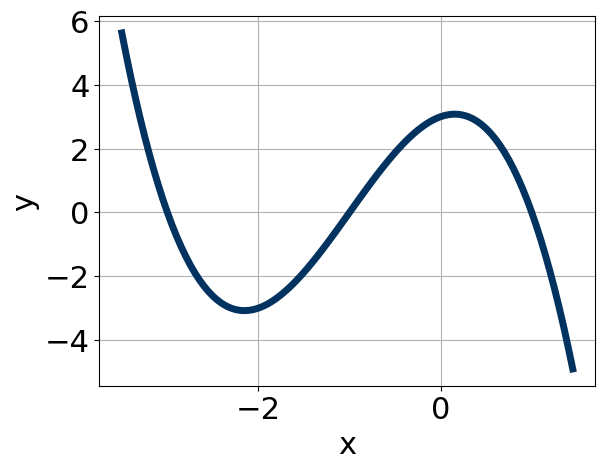
\includegraphics[width=0.5\textwidth]{../Figures/polyGraphToFunctionB.png}
\end{center}
\begin{enumerate}[label=\Alph*.]
\item \( 13(x - 1)^{4} (x + 2)^{4} (x - 3)^{10} \)
\item \( -11(x - 1)^{6} (x + 2)^{10} (x - 3)^{4} \)
\item \( -13(x - 1)^{10} (x + 2)^{4} (x - 3)^{7} \)
\item \( 9(x - 1)^{10} (x + 2)^{10} (x - 3)^{9} \)
\item \( -13(x - 1)^{6} (x + 2)^{5} (x - 3)^{11} \)

\end{enumerate} }
\end{enumerate}

\end{document}